\subsection{Firmware}

AVR is among the many architectures suported by the \texttt{gcc} compiler,
which makes it possible to write microcontroller software in C. The compiled
binary may be flashed to the chip using \texttt{avrdude}, a generic
on-chip memory uploader for AVR, paired with a hardware programmer such as
USBasp.

Conceptually, the firmware may be divided into several sections which interact
with each other at various stages of the program execution. These are:
\begin{itemize}
    \item Main section, which contains the entry point of the program and the
    main loop
    \item USART section, which contains wrappers around the serial communication
    interface exposed by the microcontroller
    \item Command section, which parses, validates and executes commands
    \item Motion section, which contains code for calculating curves and
    controlling motors
    \item Feedback section, which sends data to the controlling computer
\end{itemize}
All sections have access to a global object referred to as the \textit{machine
state}. It represents the current configuration of the CNC machine as a result
of the commands it received. It also contains the global error code, which is
used to implement a system of exceptions.

\begin{figure}[ht]
    \begin{center}
        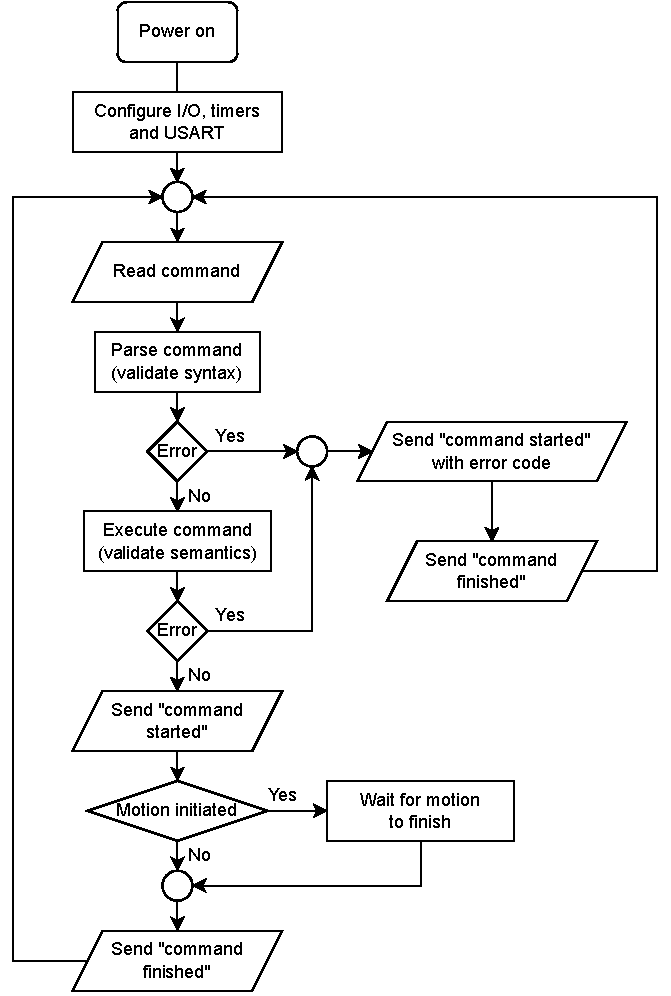
\includegraphics[width=0.47\linewidth]{firmware}
        \caption{A flowchart of the firmware's main loop.}
        \label{firmware}
    \end{center}
\end{figure}

\subsubsection{Main loop}

A key feature of the firmware is its asynchronous nature. It must simultaneously
handle serial communication, command parsing, curve calculations, and periodic
feedback. As such, the majority of the program logic is implemented by means of
interrupts, which only last for a few milliseconds before returning. All
time-sensitive operations are guaranteed to run shortly after they are invoked.

With the above in mind, the main loop serves several purposes:
\begin{enumerate}
    \item It runs time-insensitive tasks which must be executed in between
    commands (command parsing and feedback)
    \item It burns CPU cycles when no interrupts are executing
    \item It clears the global error code once feedback is sent
\end{enumerate}

Upon power-up, before the main loop is entered, configuration code is executed.
This includes setting I/O pin directions, configuring timers and USART, and
enabling interrupts.

\subsubsection{USART communication}

\begin{figure}[ht]
    \begin{center}
        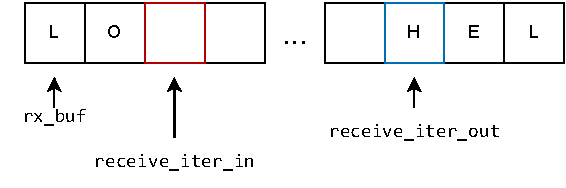
\includegraphics[width=0.6\linewidth]{usart}
        \caption{The USART circular buffer.}
        \label{firmware}
    \end{center}
\end{figure}

Receiving data is a time-sensitive operation. A byte must be collected before
the next one is received, otherwise it is lost.
